\documentclass[10pt,letterpaper]{article}
\usepackage[margin=1in]{geometry}

% https://www.overleaf.com/learn/latex/LaTeX_Graphics_using_TikZ%3A_A_Tutorial_for_Beginners_(Part_3)%E2%80%94Creating_Flowcharts
\usepackage{tikz}
\usetikzlibrary{shapes.geometric, arrows}

\author{Kyle Guarco}
\title{Homework 4 Flowchart}

\tikzstyle{startstop} = [rectangle, rounded corners,
minimum width=3cm,
minimum height=1cm,
text centered,
draw=black,
fill=red!30]

\tikzstyle{io} = [trapezium,
trapezium stretches=true, % A later addition
trapezium left angle=70,
trapezium right angle=110,
minimum width=3cm,
minimum height=1cm,
text centered,
text width=2cm,
draw=black, fill=blue!30]

\tikzstyle{process} = [rectangle,
minimum width=3cm,
minimum height=1cm,
text centered,
draw=black,
fill=orange!30]

\tikzstyle{decision} = [diamond,
minimum width=3cm,
minimum height=1cm,
text centered,
text width=2cm,
draw=black,
fill=green!30]

\tikzstyle{arrow} = [thick, ->, >=stealth]

\begin{document}
	\maketitle

	\section{Main}
	\begin{center}
		\ttfamily
		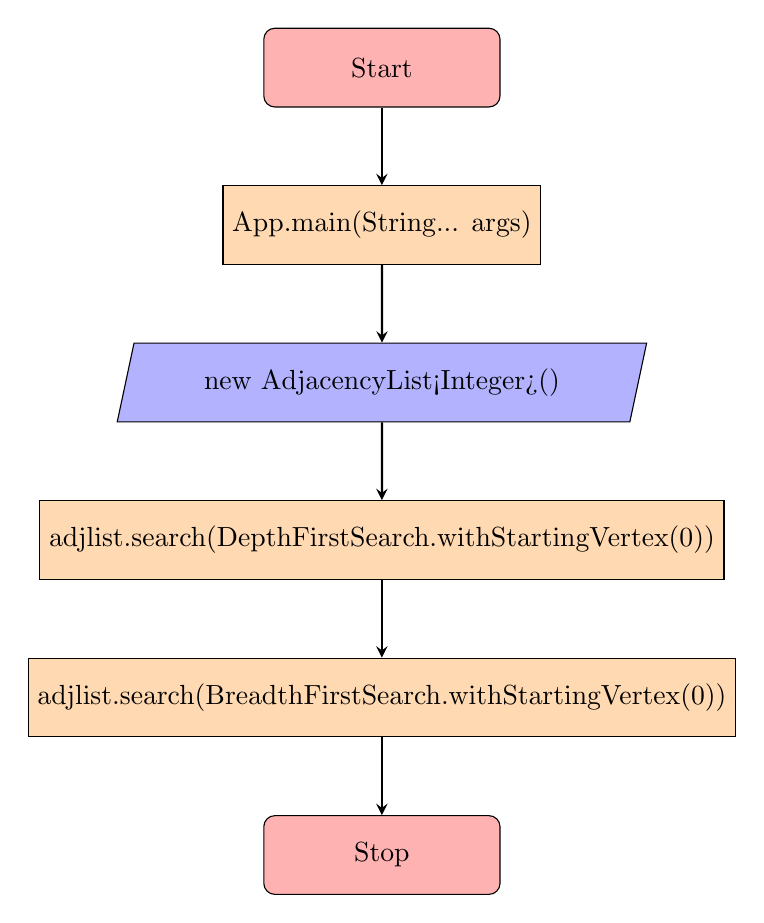
\begin{tikzpicture}[node distance=2cm]
			\node (start) [startstop] {Start};
			\node (main) [process, below of=start] {App.main(String... args)};
			\node (listnew) [io, below of=main, text width=0.5\textwidth] {new AdjacencyList<Integer>()};
			\node (dfs) [process, below of=listnew] {adjlist.search(DepthFirstSearch.withStartingVertex(0))};
			\node (bfs) [process, below of=dfs] {adjlist.search(BreadthFirstSearch.withStartingVertex(0))};
			\node (stop) [startstop, below of=bfs] {Stop};

			\draw[arrow] (start) edge (main)
							(main) edge (listnew)
							(listnew) edge (dfs)
							(dfs) edge (bfs)
							(bfs) edge (stop);
		\end{tikzpicture}
	\end{center}

	\newpage
	\section{Depth-First Search}
	\vspace{0.2in}

	\begin{center}
		\ttfamily
		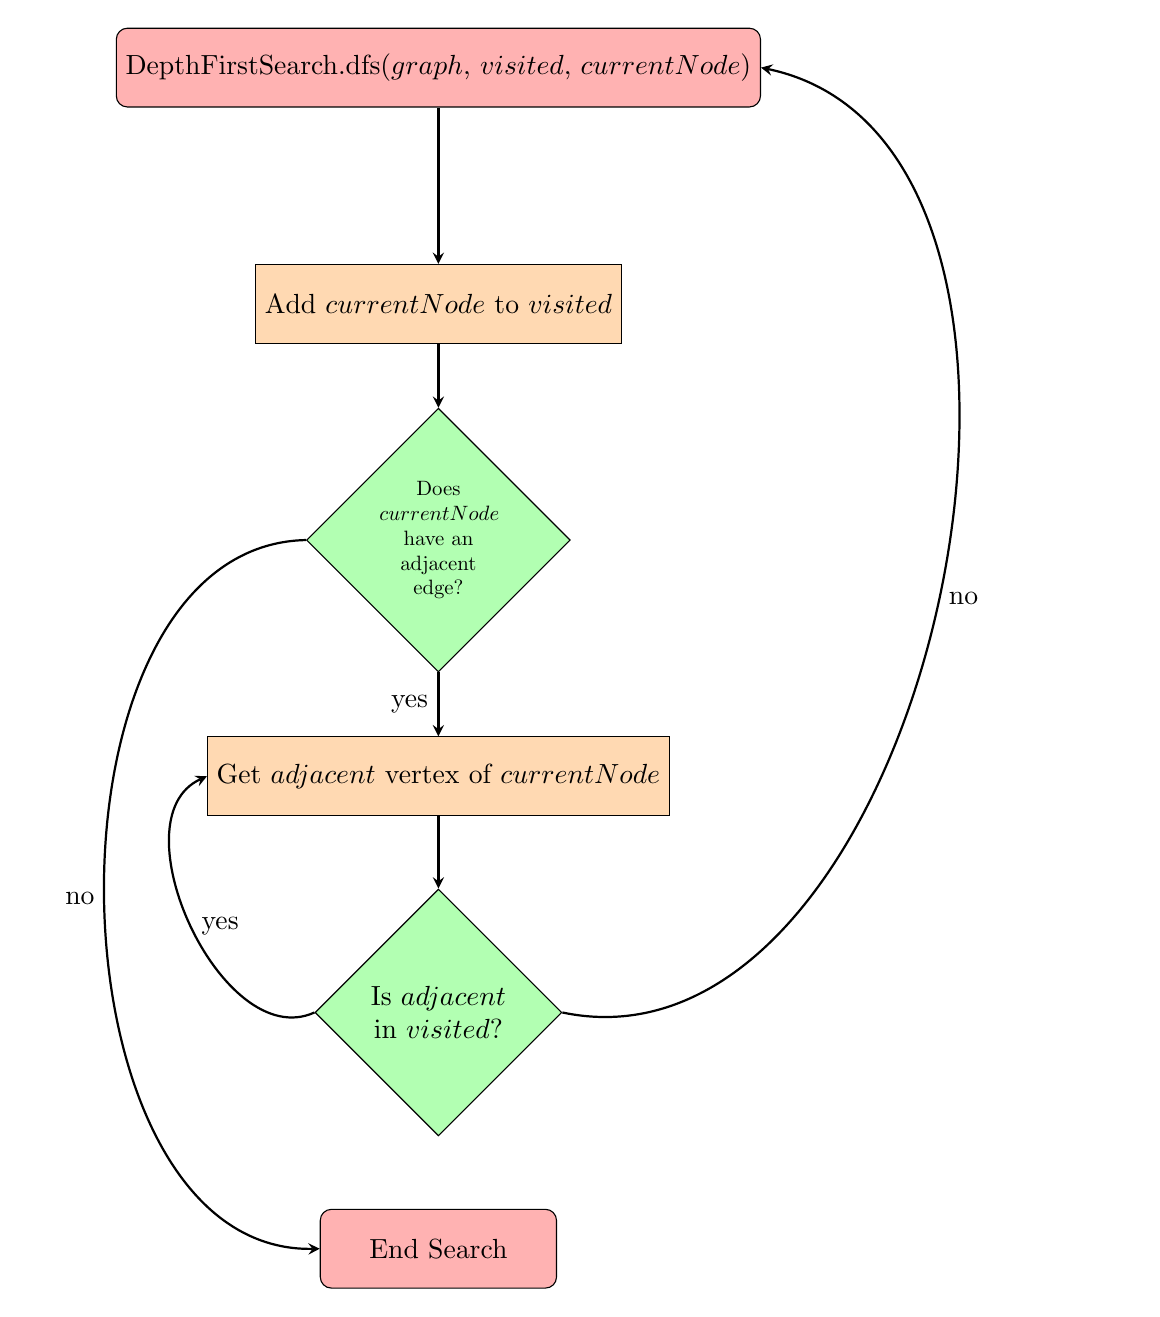
\begin{tikzpicture}[node distance=3cm]
			\node (start) [startstop] {DepthFirstSearch.dfs($graph$, $visited$, $currentNode$)};
			\node (add) [process, below of=start] {Add $currentNode$ to $visited$};
			\node (hasedge) [decision, below of=add, scale=0.75] {Does $currentNode$ have an adjacent edge?};
			\node (other) [process, below of=hasedge] {Get $adjacent$ vertex of $currentNode$};
			\node (check) [decision, below of=other] {Is $adjacent$ in $visited$?};
			\node (stop) [startstop, below of=check] {End Search};

			\draw[arrow] (start) edge (add)
							(add) edge (hasedge)
							(hasedge) edge[bend right=90] node[anchor=east] {no} (stop)
							(hasedge) edge node[anchor=east] {yes} (other)
							(other) edge (check)
							(check) edge[bend right=90] node[anchor=west] {no} (start)
							(check) edge[bend left=90] node[anchor=west] {yes} (other);
		\end{tikzpicture}
	\end{center}

	\newpage
	\section{Breadth-First Search}
	\vspace{0.2in}

	\begin{center}
		The class is created with an initial $startingVertex$.

		\ttfamily
		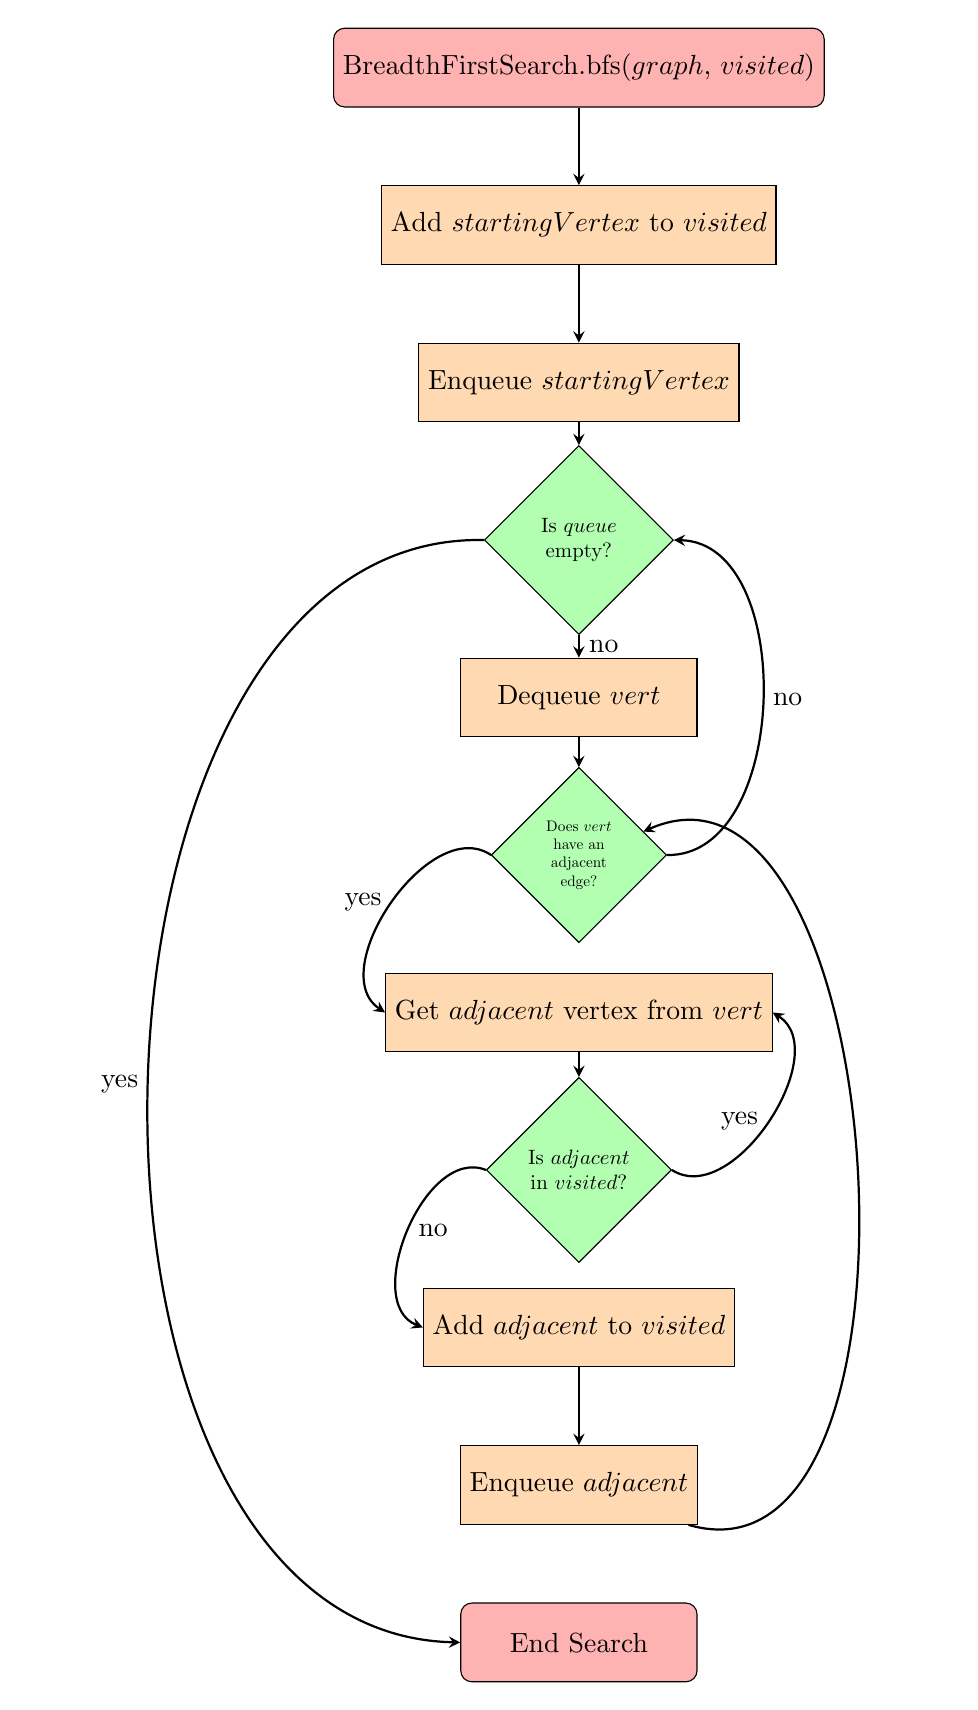
\begin{tikzpicture}[node distance=2cm]
			\node (start) [startstop] {BreadthFirstSearch.bfs($graph$, $visited$)};
			\node (add) [process, below of=start] {Add $startingVertex$ to $visited$};
			\node (starten) [process, below of=add] {Enqueue $startingVertex$};
			\node (isempty) [decision, below of=starten, scale=0.75] {Is $queue$ empty?};
			\node (vert) [process, below of=isempty] {Dequeue $vert$};
			\node (hasedge) [decision, below of=vert, scale=0.55] {Does $vert$ have an adjacent edge?};
			\node (other) [process, below of=hasedge] {Get $adjacent$ vertex from $vert$};
			\node (check) [decision, below of=other, scale=0.75] {Is $adjacent$ in $visited$?};
			\node (adjadd) [process, below of=check] {Add $adjacent$ to $visited$};
			\node (adjen) [process, below of=adjadd] {Enqueue $adjacent$};
			\node (stop) [startstop, below of=adjen] {End Search};

			\draw[arrow] (start) edge (add)
							(add) edge (starten)
							(starten) edge (isempty)
							(isempty) edge[bend right=90] node[anchor=east] {yes} (stop)
							(isempty) edge node[anchor=west] {no} (vert)
							(vert) edge (hasedge)
							(hasedge) edge[bend right=90] node[anchor=east] {yes} (other)
							(hasedge) edge[bend right=90] node[anchor=west] {no} (isempty)
							(other) edge (check)
							(check) edge[bend right=90] node[anchor=east] {yes} (other)
							(check) edge[bend right=90] node[anchor=west] {no} (adjadd)
							(adjadd) edge (adjen)
							(adjen) edge[bend right=110] (hasedge);
		\end{tikzpicture}
	\end{center}
\end{document}
